
\section{树的基本概念}

\subsection{定义和基本术语}

\begin{frame}\ft{\subsecname}
\begin{dingyi}[树-Tree]
树是$n(n\ge0)$个结点的有限集合$T$。$n=0$时称为空树。在任意一棵非空树中:
\begin{itemize}
\item[(1)]
有且只有一个特定的称为根(Root)的结点;
\item[(2)]
若$n>1$时,其余结点被分为$m(m>0)$个互不相交的子集$T_1,T_2,\cd,T_m$,其中每个子集本身又是一棵树,称其为根的子树(Subtree)。
\end{itemize}
\end{dingyi}

\end{frame}
%
\begin{frame}\ft{\subsecname}
\begin{figure}[ht!]
\centering
\begin{minipage}[t]{0.8\textwidth}
\centering
\begin{figure}
\centering
\begin{tikzpicture}[scale=0.8]

\node [below=.5] at (0,0) {(a)只有根结点};
\node [below=4] at (6,0) {(b)一般的树};

\tikzstyle{every node}=[ball color=red!70,circle,text=white]

\node [circle,draw] at (0,0) {A}; 

\node [circle,draw] at (6,0) {A}[sibling distance=2.2cm] 
  child { node[circle,draw]{B}[sibling distance=1.6cm]
	 child {node[circle,draw]{E}[sibling distance=1.5cm]
		child {node[circle,draw]{K}}
      child {node[circle,draw]{L}}
    }
	 child {node[circle,draw]{F}}      
  }
  child { node[circle,draw]{C}
    child {node[circle,draw]{G}[sibling distance=1.5cm]          
      child {node[circle,draw]{M}} 
      child {node[circle,draw]{N}}   
    }			
  }	
  child { node[circle,draw]{D}[sibling distance=1.1cm]
    child {node[circle,draw]{H}} 
    child {node[circle,draw]{I}}
    child {node[circle,draw]{J}}
  };  

\tikzstyle{every node}=[]
\tikzstyle{information text}=[rounded corners,fill=blue!20!red!40,inner sep=1ex]

\draw[xshift=-2.cm,yshift=-5.6cm]
node[below right,text width=11cm%,style=information text
]
{
 \begin{block}{结点(node)}
一个数据元素及其若干指向其子树的分支。
\end{block}
};
 
\end{tikzpicture}
\end{figure}
        
\end{minipage}
 
\begin{minipage}[t]{0.33\textwidth}
\centering
\begin{figure}
\centering
\begin{tikzpicture}[scale=0.8]

\node [below=.5] at (0,0) {(a)只有根结点};
\node [below=4] at (6,0) {(b)一般的树};

\tikzstyle{every node}=[ball color=red!70,circle,text=white]

\node [circle,draw] at (0,0) {A}; 

\node [circle,draw] at (6,0) {A}[sibling distance=2.2cm] 
  child { node[circle,draw]{B}[sibling distance=1.6cm]
	 child {node[circle,draw]{E}[sibling distance=1.5cm]
		child {node[circle,draw]{K}}
      child {node[circle,draw]{L}}
    }
	 child {node[circle,draw]{F}}      
  }
  child { node[circle,draw]{C}
    child {node[circle,draw]{G}[sibling distance=1.5cm]          
      child {node[circle,draw]{M}} 
      child {node[circle,draw]{N}}   
    }			
  }	
  child { node[circle,draw]{D}[sibling distance=1.1cm]
    child {node[circle,draw]{H}} 
    child {node[circle,draw]{I}}
    child {node[circle,draw]{J}}
  };  

\tikzstyle{every node}=[]
\tikzstyle{information text}=[rounded corners,fill=blue!20!red!40,inner sep=1ex]

\draw[xshift=-2.cm,yshift=-5.6cm]
node[below right,text width=11cm%,style=information text
]
{
 \begin{block}{结点(node)}
一个数据元素及其若干指向其子树的分支。
\end{block}
};
 
\end{tikzpicture}
\end{figure}
        
\end{minipage}\hfill
\begin{minipage}[t]{0.33\textwidth}
\centering
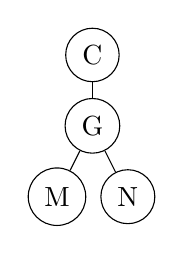
\begin{tikzpicture}[scale=0.6]  
  \node [circle,draw] at (0,0) {C}[sibling distance=1.6cm] 
  child { node[circle,draw]{G}[sibling distance=1.5cm]
    child {node[circle,draw]{M}}
    child {node[circle,draw]{N}}
  };
\end{tikzpicture}
        
\end{minipage}\hfill
\begin{minipage}[t]{0.33\textwidth}
\centering
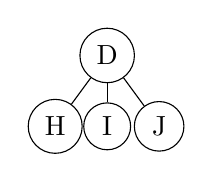
\begin{tikzpicture}[scale=0.6]
  \node [circle,draw] at (0,0) {D}[sibling distance=1.1cm] 
  child {node[circle,draw]{H}}
  child {node[circle,draw]{I}}
  child {node[circle,draw]{J}};
\end{tikzpicture}
        
\end{minipage}
\end{figure}
\end{frame}
%
\begin{frame}\ft{\subsecname}
\begin{itemize}
\item $n>0$时,根节点是唯一的,不可能存在多个根结点。\\[0.1in]
\item $m>0$时,子树的个数没有限制,但它们一定互不相交。
\end{itemize}
\end{frame}
%
\begin{frame}\ft{\subsecname}
\begin{dingyi}[结点-node]
树的结点包含一个数据元素及其若干指向其子树的分支。
\end{dingyi}
\pause 

\begin{figure}
\centering
\begin{figure}
  \centering
  \begin{tikzpicture}[scale=0.8]

    %% \tikzstyle{every node}=[ball color=red!70,circle,text=white]

    \draw[fill=red!60] (-4,2)circle(1em) node[below=1em]{根结点};
    \draw[fill=blue!60] (0,2)circle(1em) node[below=1em]{内部结点};
    \draw[] (4,2)circle(1em) node[below=1em]{叶结点或终端结点};

    \node [circle,draw,fill=red!60] at (0,0) {A}[sibling distance=2.2cm] 
    child { node[circle,draw,fill=blue!60]{B}[sibling distance=1.6cm]
      child {node[circle,draw,fill=blue!60]{E}[sibling distance=1.5cm]
	child {node[circle,draw]{K}}
        child {node[circle,draw]{L}}
      }
      child {node[circle,draw]{F}}      
    }
    child { node[circle,draw,fill=blue!60]{C}
      child {node[circle,draw,fill=blue!60]{G}[sibling distance=1.5cm]          
        child {node[circle,draw]{M}} 
        child {node[circle,draw]{N}}   
      }			
    }	
    child { node[circle,draw,fill=blue!60]{D}[sibling distance=1.1cm]
      child {node[circle,draw]{H}} 
      child {node[circle,draw]{I}}
      child {node[circle,draw]{J}}
    };  



  \end{tikzpicture}
\end{figure}

\end{figure}

\end{frame}
%

\begin{frame}\ft{\subsecname}
\begin{dingyi}[结点的度、树的度]
结点所拥有的子树的棵数称为结点的度。树中结点度的最大值称为树的度。
\end{dingyi}
\pause 

\begin{figure}
\centering
\begin{tikzpicture}[scale=0.8]
  %% \tikzstyle{every node}=[ball color=red!70,circle,text=white]


  \node [below right,circle,draw] at (2,0) {A}[sibling distance=2.2cm] 
  child { node[circle,draw]{B}[sibling distance=1.6cm]
    child {node[circle,draw]{E}[sibling distance=1.5cm]
      child {node[circle,draw]{K}}
      child {node[circle,draw]{L}}
    }
    child {node[circle,draw]{F}}      
  }
  child { node[circle,draw]{C}
    child {node[circle,draw]{G}[sibling distance=1.5cm]          
      child {node[circle,draw]{M}} 
      child {node[circle,draw]{N}}   
    }			
  }	
  child { node[circle,draw]{D}[sibling distance=1.1cm]
    child {node[circle,draw]{H}} 
    child {node[circle,draw]{I}}
    child {node[circle,draw]{J}}
  };  
  
  \tikzstyle{information text}=[rounded corners,fill=blue!40!red!40,inner sep=1ex]
  \draw[xshift=6.cm,yshift=0cm]
  node[below right,text width=4.8cm,style=information text]
  {
    A的度为3,B的度为2,M的度为0,树的度为3.
  };
  
\end{tikzpicture}

\end{figure}


\end{frame}

\begin{frame}\ft{\subsecname}
\begin{dingyi}[叶子结点、分支结点]
度为0的结点称为\textcolor{acolor5}{叶子结点};
度不为0的结点称为\textcolor{acolor5}{分支结点}。
除根结点外,分支结点又称为内部结点。
\end{dingyi}
\pause 

\begin{figure}
\centering
\begin{tikzpicture}[scale=0.8]

  %% \tikzstyle{every node}=[ball color=red!70,circle,text=white]

  \node [below right,circle,draw] at (2,0) {A}[sibling distance=2.2cm] 
  child { node[circle,draw]{B}[sibling distance=1.6cm]
    child {node[circle,draw]{E}[sibling distance=1.5cm]
      child {node[circle,draw]{K}}
      child {node[circle,draw]{L}}
    }
    child {node[circle,draw]{F}}      
  }
  child { node[circle,draw]{C}
    child {node[circle,draw]{G}[sibling distance=1.5cm]          
      child {node[circle,draw]{M}} 
      child {node[circle,draw]{N}}   
    }			
  }	
  child { node[circle,draw]{D}[sibling distance=1.1cm]
    child {node[circle,draw]{H}} 
    child {node[circle,draw]{I}}
    child {node[circle,draw]{J}}
  };  

  \tikzstyle{every node}=[]
  \tikzstyle{information text}=[rounded corners,fill=blue!40!red!40,inner sep=1ex]
  \draw[xshift=6.cm,yshift=0cm]
  node[below right,text width=4.8cm,style=information text]
  {
    H、I、J、K、L、M、N是叶子结点,而所有其它结点都是分支结点。
  };
  
\end{tikzpicture}

\end{figure}


\end{frame}



\begin{frame}\ft{\subsecname}
\begin{dingyi}[孩子结点、双亲结点、兄弟结点]
结点的子树的根称为该结点的\textcolor{acolor5}{孩子(child)},相应地,该结点是其孩子结点的\textcolor{acolor5}{双亲(parent)}。同一双亲的所有子结点互称\textcolor{acolor5}{兄弟(sibling)}。
\end{dingyi}

\begin{figure}
\centering
\begin{tikzpicture}[scale=0.8]

%% \tikzstyle{every node}=[ball color=red!70,circle,text=white]

\node[below right,circle,draw] at (2,0) {A}[sibling distance=2.2cm] 
  child { node[circle,draw]{B}[sibling distance=1.6cm]
	 child {node[circle,draw]{E}[sibling distance=1.5cm]
		child {node[circle,draw]{K}}
      child {node[circle,draw]{L}}
    }
	 child {node[circle,draw]{F}}      
  }
  child { node[circle,draw]{C}
    child {node[circle,draw]{G}[sibling distance=1.5cm]          
      child {node[circle,draw]{M}} 
      child {node[circle,draw]{N}}   
    }			
  }	
  child { node[circle,draw]{D}[sibling distance=1.1cm]
    child {node[circle,draw]{H}} 
    child {node[circle,draw]{I}}
    child {node[circle,draw]{J}}
  };  

\tikzstyle{every node}=[]
\tikzstyle{information text}=[rounded corners,fill=blue!40!red!40,inner sep=1ex]
\draw[xshift=6.2cm,yshift=0cm]
node[below right,text width=4.6cm,style=information text]
{
B 、C、D是A的孩子,而A是B 、C、D的双亲;类似地,E 、F是B的孩子,B是E 、F的双亲。
B 、C、D互为兄弟;E 、F互为兄弟。

};
 
\end{tikzpicture}
    
\end{figure}
\end{frame}
%
\begin{frame}\ft{\subsecname}
\begin{dingyi}[层次、堂兄弟结点]
结点的\textcolor{acolor5}{层次(level)}从根开始定义,根为第1层,根的孩子为第2层。若某结点在第$l$层,则其子树的根就在第$l+1$层。 双亲在同一层上的结点互为\textcolor{acolor5}{堂兄弟}。
\end{dingyi}

\begin{figure}
\centering
\begin{tikzpicture}[scale=0.8]

%% \tikzstyle{every node}=[ball color=red!70,circle,text=white]

\node[below right,circle,draw] at (2,0) {A}[sibling distance=2.2cm] 
  child { node[circle,draw]{B}[sibling distance=1.6cm]
	 child {node[circle,draw]{E}[sibling distance=1.5cm]
		child {node[circle,draw]{K}}
      child {node[circle,draw]{L}}
    }
	 child {node[circle,draw]{F}}      
  }
  child { node[circle,draw]{C}
    child {node[circle,draw]{G}[sibling distance=1.5cm]          
      child {node[circle,draw]{M}} 
      child {node[circle,draw]{N}}   
    }			
  }	
  child { node[circle,draw]{D}[sibling distance=1.1cm]
    child {node[circle,draw]{H}} 
    child {node[circle,draw]{I}}
    child {node[circle,draw]{J}}
  };  

\tikzstyle{every node}=[]
\tikzstyle{information text}=[rounded corners,fill=blue!40!red!40,inner sep=1ex]
\draw[xshift=6.2cm,yshift=0cm]
node[below right,text width=4.6cm,style=information text]
{
E、F、G、H、I、J互为为堂兄弟。
};
 
\end{tikzpicture}
    
\end{figure}
\end{frame}
%
%
\begin{frame}\ft{\subsecname}
\begin{dingyi}[结点的层次路径、祖先、子孙]
从根结点开始,到达某结点p所经过的所有结点构成结点p的\textcolor{acolor5}{层次路径}(有且只有一条)。结点p的层次路径上的所有结点(p除外)称为p的\textcolor{acolor5}{祖先(ancester)} 。以某一结点为根的子树中的任意结点称为该结点的\textcolor{acolor5}{子孙结点(descent)}。
\end{dingyi}
\end{frame}
%
%
\begin{frame}\ft{\subsecname}
\begin{figure}
\centering
\begin{tikzpicture}[scale=0.8]

%% \tikzstyle{every node}=[ball color=red!70,circle,text=white]

\node[below right,circle,draw] at (2,0) {A}[sibling distance=2.2cm] 
  child { node[circle,draw]{B}[sibling distance=1.6cm]
	 child {node[circle,draw]{E}[sibling distance=1.5cm]
		child {node[circle,draw]{K}}
      child {node[circle,draw]{L}}
    }
	 child {node[circle,draw]{F}}      
  }
  child { node[circle,draw]{C}
    child {node[circle,draw]{G}[sibling distance=1.5cm]          
      child {node[circle,draw]{M}} 
      child {node[circle,draw]{N}}   
    }			
  }	
  child { node[circle,draw]{D}[sibling distance=1.1cm]
    child {node[circle,draw]{H}} 
    child {node[circle,draw]{I}}
    child {node[circle,draw]{J}}
  };  

\tikzstyle{every node}=[]
\tikzstyle{information text}=[rounded corners,fill=blue!40!red!40,inner sep=1ex]
\draw[xshift=6.2cm,yshift=0cm]
node[below right,text width=4.6cm,style=information text]
{
 K的层次路径为: A、B、E、K。

A、B、E为K的祖先。
};
 
\end{tikzpicture}
    
\end{figure}
\end{frame}


\begin{frame}\ft{\subsecname}
\begin{dingyi}[树的深度-depth]
树中结点的最大层次值,又称为树的\textcolor{acolor5}{高度}。
\end{dingyi}
\begin{tikzpicture}[scale=0.8]

%% \tikzstyle{every node}=[ball color=red!70,circle,text=white]

\node[below right,circle,draw] at (2,0) {A}[sibling distance=2.2cm] 
  child { node[circle,draw]{B}[sibling distance=1.6cm]
	 child {node[circle,draw]{E}[sibling distance=1.5cm]
		child {node[circle,draw]{K}}
      child {node[circle,draw]{L}}
    }
	 child {node[circle,draw]{F}}      
  }
  child { node[circle,draw]{C}
    child {node[circle,draw]{G}[sibling distance=1.5cm]          
      child {node[circle,draw]{M}} 
      child {node[circle,draw]{N}}   
    }			
  }	
  child { node[circle,draw]{D}[sibling distance=1.1cm]
    child {node[circle,draw]{H}} 
    child {node[circle,draw]{I}}
    child {node[circle,draw]{J}}
  };  

\tikzstyle{every node}=[]
\tikzstyle{information text}=[rounded corners,fill=blue!40!red!40,inner sep=1ex]
\draw[xshift=6.2cm,yshift=0cm]
node[below right,text width=4.6cm,style=information text]
{
该树的高度为4.
};
 
\end{tikzpicture}
    
\begin{figure}
\centering

\end{figure}
\end{frame}
%
%
\begin{frame}\ft{\subsecname}
\begin{dingyi}[有序树和无序树]
对于一棵树,若其中每一个结点的子树具有一定的次序,则该树称为\textcolor{acolor5}{有序树},否则称为\textcolor{acolor5}{无序树}。
\end{dingyi}

\begin{dingyi}[森林-forest]
\textcolor{acolor5}{森林}是$m(m\ge0)$棵互不相交的树的集合。显然,若将一棵树的根结点删除,剩余的子树就构成了森林。
\end{dingyi}
\end{frame}
%
\subsection{树的表示形式}
\begin{frame}\ft{树的表示形式}
1、倒悬树
\begin{figure}
\centering
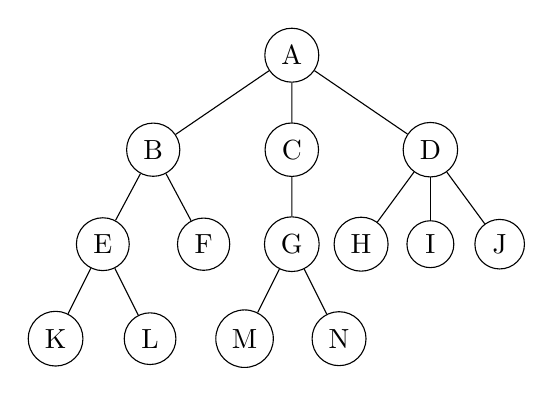
\begin{tikzpicture}[scale=0.8]

%% \tikzstyle{every node}=[ball color=red!70,circle,text=white]

\node[below right,circle,draw] at (2,0) {A}[sibling distance=2.2cm] 
  child { node[circle,draw]{B}[sibling distance=1.6cm]
	 child {node[circle,draw]{E}[sibling distance=1.5cm]
		child {node[circle,draw]{K}}
      child {node[circle,draw]{L}}
    }
	 child {node[circle,draw]{F}}      
  }
  child { node[circle,draw]{C}
    child {node[circle,draw]{G}[sibling distance=1.5cm]          
      child {node[circle,draw]{M}} 
      child {node[circle,draw]{N}}   
    }			
  }	
  child { node[circle,draw]{D}[sibling distance=1.1cm]
    child {node[circle,draw]{H}} 
    child {node[circle,draw]{I}}
    child {node[circle,draw]{J}}
  };  

%% \tikzstyle{every node}=[]
%\tikzstyle{information text}=[rounded corners,fill=blue!40!red!40,inner sep=1ex]
%\draw[xshift=6.2cm,yshift=0cm]
%node[below right,text width=4.6cm,style=information text]
%{
%该树的高度为4.
%};
% 
\end{tikzpicture}
    
\end{figure}

\end{frame}
%
\begin{frame}\ft{树的表示形式}
2、嵌套集合

\begin{figure}
\centering
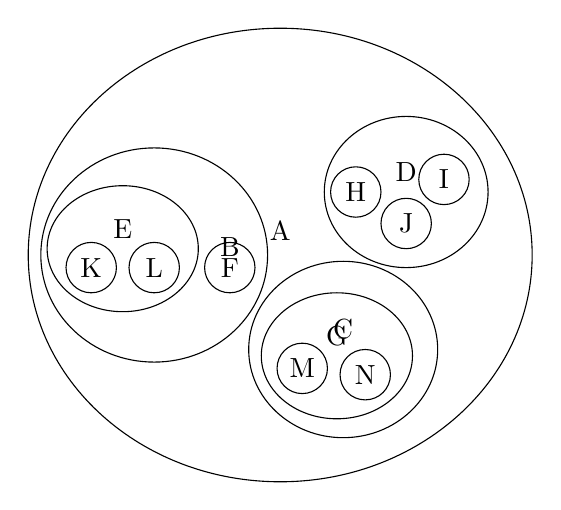
\begin{tikzpicture}[scale=0.8]
\draw (0,0)node[above=1.8]{A} ellipse (4cm and 3.6cm);
\draw (-2,0) ellipse (1.8cm and 1.7cm);
\draw (-2.5,0.1)node[above=0.2]{E} ellipse (1.2cm and 1cm);
\draw (-3,-0.2)node[]{K} circle(0.4);
\draw (-2,-0.2)node[]{L} circle(0.4);
\draw (-0.8,-0.2)node[]{F} circle(0.4) node[above=0.4]{B};

\draw (2,1)node[above=0.3]{D} ellipse (1.3cm and 1.2cm);
\draw (1.2,1)node[]{H} circle(0.4);
\draw (2.6,1.2)node[]{I} circle(0.4);
\draw (2,0.5)node[]{J} circle(0.4);


\draw (1,-1.5)node[above=0.6]{C} ellipse (1.5cm and 1.4cm);
\draw (0.9,-1.6)node[above=0.1]{G} ellipse (1.2cm and 1cm);
\draw (0.35,-1.8)node[]{M} circle(0.4);
\draw (1.35,-1.9)node[]{N} circle(0.4);

\end{tikzpicture}
    
\end{figure}

\end{frame}
%
\begin{frame}\ft{树的表示形式}
3、 广义表形式

$$
\mbox{(A(B(E(K,L),F), C(G(M,N)), D(H,I,J)))}
$$
\end{frame}
%
\begin{frame}\ft{线性结构与树型结构的区别}
\textcolor{acolor5}{线性结构}
\begin{itemize}
\item 第一个元素:无前驱
\item 最后一个元素:无后继
\item 中间元素:一个直接前驱和一个直接后继
\end{itemize}
 
\textcolor{acolor5}{树结构}
\begin{itemize}
\item 根结点:无双亲,且唯一
\item 叶结点:无孩子,不唯一
\item 中间结点:一个双亲多个孩子
\end{itemize}
\end{frame}

\subsection{树的抽象数据类型}
\begin{frame}[fragile]\ft{树的抽象数据类型}
\begin{lstlisting}[basicstyle=\ttfamily\footnotesize]
ADT Tree{
Data:
`树由一个根结点和若干棵子树构成。结点有相同数据类型及层次关系。`
Operation:
  Init(*T): 
  Clear(*T):
  Creat(*T):  
  IsEmpty(T):
  Depth(T):
  Root(T):
  Value(T, e):
  Assign(T, e, value):
  ...
} ADT Tree
\end{lstlisting}
\end{frame}
